\documentclass[12pt]{article}
\usepackage{graphicx}
\usepackage{longtable}
\usepackage{listings}
\usepackage[letterpaper, margin=2cm]{geometry}
\usepackage[T1]{fontenc}
\usepackage{polski}
\usepackage[export]{adjustbox}
\usepackage[utf8]{inputenc}
\usepackage[polish]{babel}
\graphicspath{{.}}
\usepackage{tocloft}
\usepackage{hyperref}

\hypersetup{%
    colorlinks,
    citecolor=black,
    filecolor=black,
    linkcolor=black,
    urlcolor=black
}

\renewcommand{\cftsecleader}{\cftdotfill{\cftdotsep}}

\lstset{
    postbreak=\mbox{\textcolor{red}{$\hookrightarrow$}\space}
    belowcaptionskip=1\baselineskip,
    breaklines=true,
    frame=L,
    numbers=left,
    xleftmargin=\parindent,
    language=bash,
    showstringspaces=false,
    basicstyle=\footnotesize\ttfamily,
    identifierstyle=\color{blue},
    stringstyle=\color{orange},
}

\begin{document}
    \centering
    
\includegraphics[width=5cm, height=5cm,]{herbPL.jpg}
    \hspace{2cm}
    
\includegraphics[width=5cm, height=5cm]{herbWEII.jpg}\\
    \vspace{2cm}
    {\Huge \textbf{SPRAWOZDANIE}}
    \vspace{2cm}
    \newline
    {\large PROGRAMOWANIE W CHMURZE OBLICZENIOWEJ}
    \vfill

    \raggedright{}

    \textbf{IMIĘ I NAZWISKO:} Piotr Czajka

    \textbf{NUMER LABORATORIUM} 3\\
    \textbf{GRUPA:} 7.1.2\\
    \textbf{Data wykonywania ćwiczenia:} 25.10.2018\\

    \newpage

    \tableofcontents{}

    \newpage

    \section{Cel laboratorium}
    Celem laboratorium było zapoznanie się z narzędziem docker-compose, cytując z oficjalnej strony, ``Narzędzia do definiowania i uruchamiania wielokontenerowych aplikacji Docker''\

    \section{Przebieg ćwiczenia}

    \subsection{Zadanie pierwsze}

    Najpierw upewniam się, że docker-compose jest zainstalowany:

    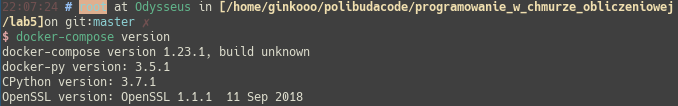
\includegraphics[width=\textwidth]{1_1.png}

    Teraz odpalam kontener z ghostem, aby później skopiować jego domyślną konfigurację na dysk i ją zmodyfikować:

    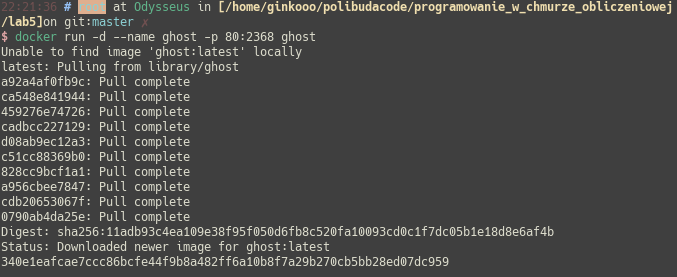
\includegraphics[width=\textwidth]{1_2.png}

    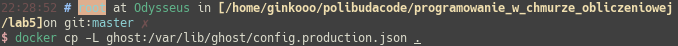
\includegraphics[width=\textwidth]{1_3.png}

    \subsection{Zadanie drugie}

    Jak widać serwer działa, na razie korzysta z sqlite jako bazy danych:

    
\includegraphics[width=\textwidth]{1_4.png}

    Tak zmodyfikowałem config.production.json, aby korzystał z bazy mysql: (zmiana dotyczyła sekcji ``database'')

    \lstinputlisting{config.production.json}

    Utworzyłem taki oto Dockerfile, aby przy buildzie kopiował zmodyfikowany config do odpowiedniego katalogu:

    \lstinputlisting{Dockerfile}

    Teraz przyszła kolej na stworzenie odpowiedniego docker-compose:

    \lstinputlisting{docker-compose.yml}

    Mysql działa domyślnie na porcie 3306, więc otwieramy go, w sekcji enviroment konfigurujemy dane dostępowe do mysql. restart: on-failure ma za zadanie restartować serwer Ghosta, aż nie uda mu się połączyć z mysql, który startuje dość długo. Nie wystaraczy sama dyrektywa depends\_on, ponieważ mysql włącza się, ale dopiero jakiś czas po włączeniu serwer jest dostępny, by się z nim łączyć.

\end{document}
